\section{Spatial proteomics}

\begin{frame}{}
  \begin{center}
    \Large{\textbf{Use case}: spatial proteomics.}
  \end{center}
\end{frame}

\subsection*{The LOPIT pipeline}

\label{sec:spintro}

%% \begin{frame}{Regulations}
%%   \begin{figure}[h]
%%     \centering
%%     \includegraphics[width=1\linewidth]{Figures2/regulation.jpg}
%%   \end{figure}
%% \end{frame}

\label{sec:spspatprot}

\begin{frame}{Cell organisation - regulation of protein localisation}
  \begin{center}
    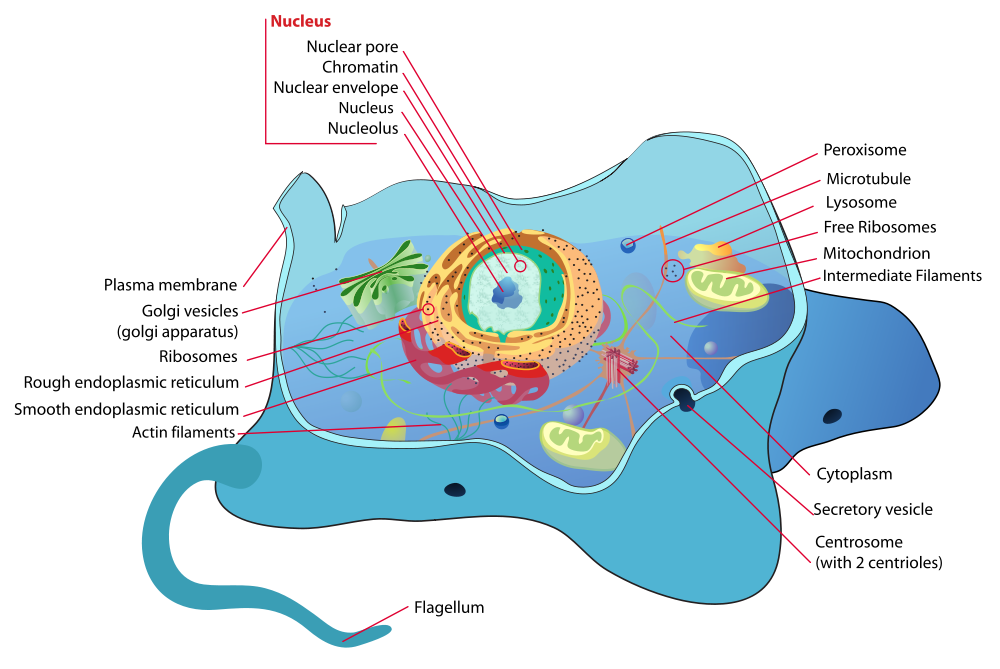
\includegraphics[width=1\linewidth]{Figures/Animal_cell_structure.png} \\
    \textbf{\textcolor{Blue}{Spatial proteomics}} is the systematic
    study of protein localisations.
  \end{center}

  \tiny Image from Wikipedia
  \url{http://en.wikipedia.org/wiki/Cell_(biology)}.
\end{frame}

% \begin{frame}{Spatial proteomics - Why?}
%   \begin{itemize}
%   \item Localisation is function
%   \item Mis-localisation \citep{Kau2004,Laurila2009}
%   \item Re-localisation
%   \end{itemize}
% \end{frame}

\begin{frame}{Spatial proteomics - Why?}
  \begin{block}{Localisation is function}
    \begin{itemize}
    \item The cellular sub-division allows cells to establish a range
      of distinct micro-environments, each favouring different
      biochemical reactions and interactions and, therefore, allowing
      each compartment to fulfil a particular functional role.
    \item Localisation and sequestration of proteins within
      sub-cellular niches is a fundamental mechanism for the
      post-translational regulation of protein function.
    \end{itemize}
  \end{block}
  \begin{block}{Re-localisation in}
    \begin{itemize}
    \item \textcolor{Blue}{Differentiation} stem cells.
    \item \textcolor{Blue}{Activation} of biological processes.
    \end{itemize}
    %% Examples later.
  \end{block}
\end{frame}

\begin{frame}{Spatial proteomics - Why?}
  \begin{block}{Mis-localisation}
    Disruption of the targeting/trafficking process alters proper
    sub-cellular localisation, which in turn perturb the cellular
    functions of the proteins.
    \begin{itemize}
    \item Abnormal protein localisation leading to the \textbf{loss of
        functional} effects in diseases \citep{Laurila2009}.
    \item Disruption of the nuclear/cytoplasmic transport (nuclear
      pores) have been detected in many types of \textbf{carcinoma
        cells} \citep{Kau2004}.
    \item Sub-cellular localisation of MC4R with ADCY3 at neuronal
      primary cilia underlies a common pathway for genetic
      predisposition to \textbf{obesity} \citep{Siljee:2018}.
    \end{itemize}
  \end{block}

\end{frame}


\subsubsection*{Experimental designs}
\label{sec:expdesign}

\begin{frame}{Spatial proteomics - How, experimentally}
  \begin{figure}
    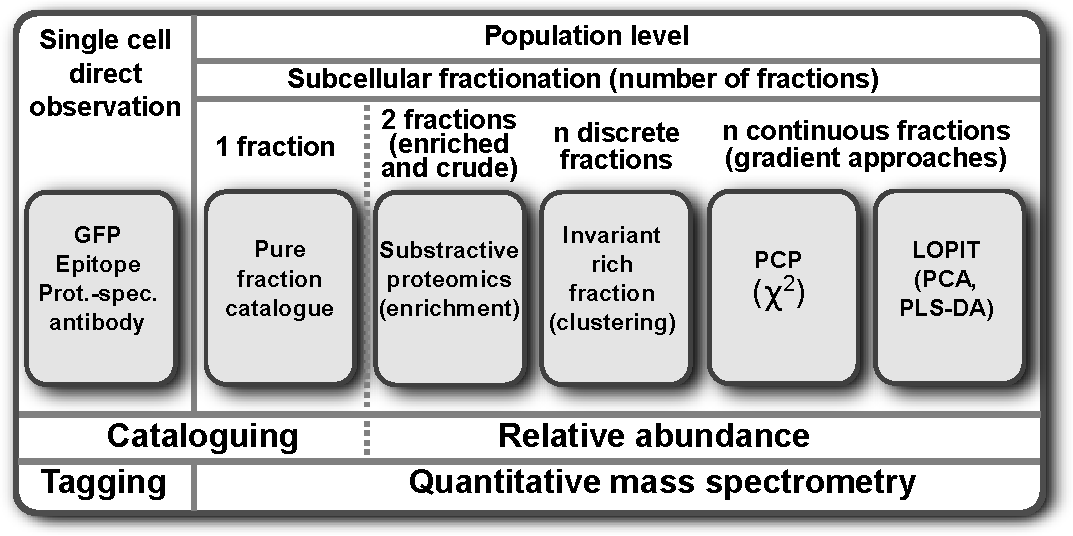
\includegraphics[width=.8\linewidth]{Figures/F02-expdesigns.pdf}
    \caption{Organelle proteomics approaches \citep{Gatto:2010}}
  \end{figure}
\end{frame}

\begin{frame}{Fusion proteins and immunofluorescence}

  \begin{figure}[h]
    \centering
    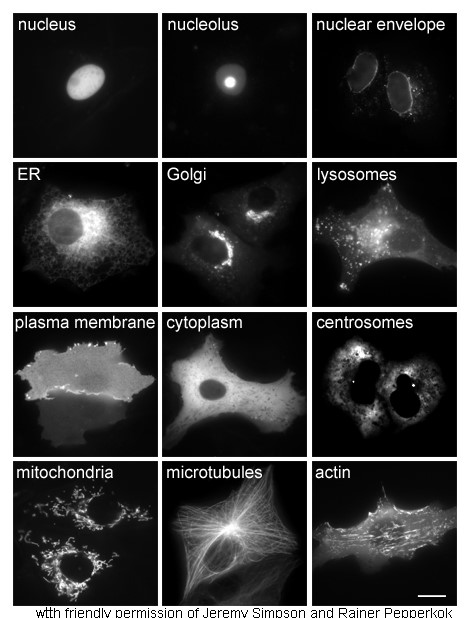
\includegraphics[width=.35\linewidth]{Figures2/Localisations02eng.jpg}
    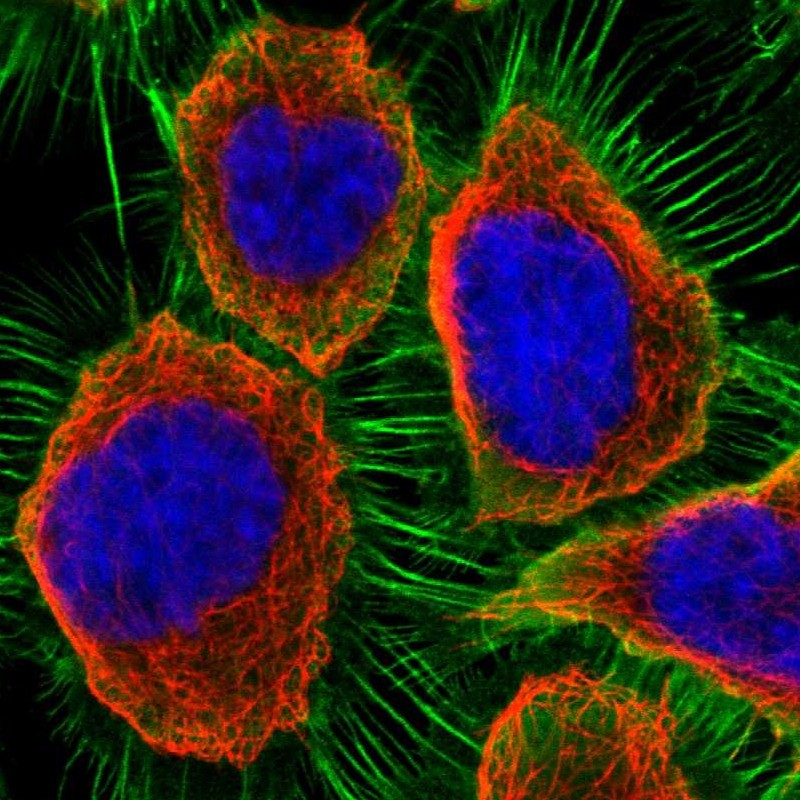
\includegraphics[width=.45\linewidth]{figures/if_selected.jpg}
    \caption{Targeted protein localisation. Example of discrepancies
      between IF and FPs as well as between FP tagging at the N and C
      termini \citep{Stadler:2013}.}
  \end{figure}
\end{frame}


\subsubsection*{Gradient approaches}
\label{sec:grad}

\begin{frame}{Spatial proteomics - How, experimentally}
  \begin{figure}
    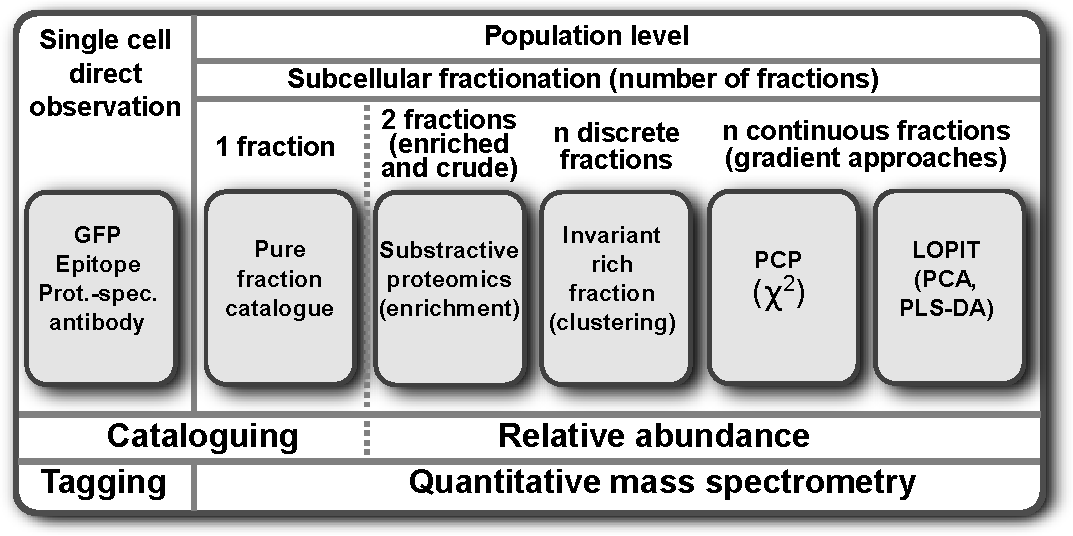
\includegraphics[width=.8\linewidth]{Figures/F02-expdesigns.pdf}
    \caption{Organelle proteomics approaches
      \citep{Gatto:2010}.}
  \end{figure}

  \textbf{Gradient approaches}: \cite{Dunkley:2006},
  \cite{Foster2006}.

  \bigskip

  \textbf{Explorative/discovery approaches},
  \textcolor{Blue}{steady-state \textbf{global localisation maps}}.
\end{frame}


\begin{frame}{}
  \begin{figure}
    % \includegraphics[width=.8\linewidth]{Figures/F03-protocols-8plex.pdf}
    % \includegraphics[width=.5\linewidth]{figures/expdesign.pdf}
    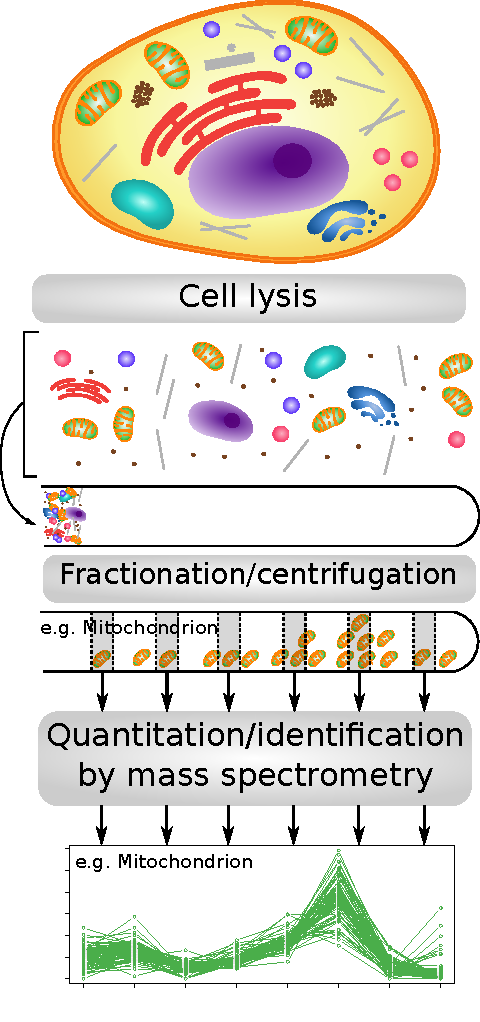
\includegraphics[width=.39\linewidth]{figures/workflow_primary.pdf}
  \end{figure}
\end{frame}

\subsubsection*{The data}
\label{sec:data}

\begin{frame}{Quantitation data}
  \begin{center}
    \begin{tabular}{|l|llll|}
      \hline
      & Fraction$_{\text{1}}$ & Fraction$_{\text{2}}$ & \ldots{} & Fraction$_{\text{m}}$ \\
      \hline
      p$_{\text{1}}$ & q$_{\text{1,1}}$ & q$_{\text{1,2}}$ & \ldots{} & q$_{\text{1,m}}$ \\
      p$_{\text{2}}$ & q$_{\text{2,1}}$ & q$_{\text{2,2}}$ & \ldots{} & q$_{\text{2,m}}$ \\
      p$_{\text{3}}$ & q$_{\text{3,1}}$ & q$_{\text{3,2}}$ & \ldots{} & q$_{\text{3,m}}$ \\
      p$_{\text{4}}$ & q$_{\text{4,1}}$ & q$_{\text{4,2}}$ & \ldots{} & q$_{\text{4,m}}$ \\
      \vdots & \vdots & \vdots & \vdots & \vdots \\
      p$_{\text{j}}$ & q$_{\text{j,1}}$ & q$_{\text{j,2}}$ & \ldots{} & q$_{\text{j, m}}$ \\
      \hline
    \end{tabular}
  \end{center}
\end{frame}

\begin{frame}{Quantitation data and organelle markers}
  \begin{center}
    \begin{tabular}{|l|llll||l|}
      \hline
      & Fraction$_{\text{1}}$ & Fraction$_{\text{2}}$ & \ldots{} & Fraction$_{\text{m}}$ & markers\\
      \hline
      p$_{\text{1}}$ & q$_{\text{1,1}}$ & q$_{\text{1,2}}$ & \ldots{} & q$_{\text{1,m}}$ & unknown \\
      p$_{\text{2}}$ & q$_{\text{2,1}}$ & q$_{\text{2,2}}$ & \ldots{} & q$_{\text{2,m}}$ & \textcolor{Red}{$loc_{1}$}\\
      p$_{\text{3}}$ & q$_{\text{3,1}}$ & q$_{\text{3,2}}$ & \ldots{} & q$_{\text{3,m}}$ & unknown \\
      p$_{\text{4}}$ & q$_{\text{4,1}}$ & q$_{\text{4,2}}$ & \ldots{} & q$_{\text{4,m}}$ & \textcolor{Blue}{$loc_{i}$}\\
      \vdots & \vdots & \vdots & \vdots & \vdots & \vdots\\
      p$_{\text{j}}$ & q$_{\text{j,1}}$ & q$_{\text{j,2}}$ & \ldots{} & q$_{\text{j, m}}$ & unknown \\
      \hline
    \end{tabular}
  \end{center}
\end{frame}
